\documentclass{article}
\usepackage{nips_2018}
\usepackage[utf8]{inputenc} % allow utf-8 input
\usepackage[T1]{fontenc}    % use 8-bit T1 fonts
\usepackage{hyperref}       % hyperlinks
\usepackage{url}            % simple URL typesetting
\usepackage{booktabs}       % professional-quality tables
\usepackage{amsfonts}       % blackboard math symbols
\usepackage{nicefrac}       % compact symbols for 1/2, etc.
\usepackage{microtype}      % microtypography
\usepackage{graphicx}
\usepackage{caption}
\usepackage{subcaption}
\usepackage{amsmath}
\usepackage{xcolor}

\title{Formatting instructions for NIPS 2018}

% The \author macro works with any number of authors. There are two
% commands used to separate the names and addresses of multiple
% authors: \And and \AND.
%
% Using \And between authors leaves it to LaTeX to determine where to
% break the lines. Using \AND forces a line break at that point. So,
% if LaTeX puts 3 of 4 authors names on the first line, and the last
% on the second line, try using \AND instead of \And before the third
% author name.

\author{
  David S.~Hippocampus\thanks{Use footnote for providing further
    information about author (webpage, alternative
    address)---\emph{not} for acknowledging funding agencies.} \\
  Department of Computer Science\\
  Cranberry-Lemon University\\
  Pittsburgh, PA 15213 \\
  \texttt{hippo@cs.cranberry-lemon.edu} \\
  %% examples of more authors
  %% \And
  %% Coauthor \\
  %% Affiliation \\
  %% Address \\
  %% \texttt{email} \\
  %% \AND
  %% Coauthor \\
  %% Affiliation \\
  %% Address \\
  %% \texttt{email} \\
  %% \And
  %% Coauthor \\
  %% Affiliation \\
  %% Address \\
  %% \texttt{email} \\
  %% \And
  %% Coauthor \\
  %% Affiliation \\
  %% Address \\
  %% \texttt{email} \\
}

\begin{document}
% \nipsfinalcopy is no longer used

\maketitle


\begin{abstract}
  We can meet thousands of people in our life. To recognize all of these people, a complex model which is able to classify all these people are needed. However, in a particular environment, like our home or office, only less than ten people appears. Thus a smaller model could be sufficient for recognition in this scenario. Assuming the number of classes and class distribution are fixed, the question is how to use this information? In recent works, transfer learning shows benefit and becomes the dominant method. We shown intrinsic problems of using transfer learning in this scenario. Instead of retraining, we brought up a method, called the probability layer, which can avoid retraining totally and performs better than transfer learning.
\end{abstract}


\section{Introduction}
% First paragraph: CNN performs very well at lab setting
Convolutional neural network (CNN) plays an important role in image recognition. In 2012, AlexNet \cite{krizhevsky2012imagenet} achieved a top-5 error of 17\% on ImageNet \cite{deng2009imagenet}, while previous method could only achieve a top-5 error of 25.7\%. Since then, CNNs have become the dominant method and main research direction in image recognition. In 2015, ResNet \cite{he2016deep} achieves a top-5 error of 3.57\%. Considering that the estimated human classification error on ImageNet is 5.1\% \cite{russakovsky2015imagenet}, we can conclude that CNNs have gained the ability of performing better than human.



% Second paragraph: When we want to use CNNs in realistic setting, many problems appear and give us chance to optimize model. The question is, how to use this information?
However, all of these results are gained in lab setting, which is different from image recognition in real life. In lab, we use shared benchmark to train and test our dataset, like ImageNet. ImageNet dataset plays an important role in the advancement of CNN models and the huge number of images in ImageNet makes it possible to train complex models with millions of parameters \cite{simonyan2014very, szegedy2015going, huang2017densely}. There are $1000$ classes in ImageNet, $1.2$ million training images and the number of training images in each class is almost equal. However, in real life, the appearance of classes has strong time and spatial locality. Even if we can meet thousands of people in our life, only less than ten people would appear in a particular environment, like our home or office. Experiments on videos of day-to-day life from Youtube \cite{shen2017fast} shows that $10$ objects comprised $90$\% of all objects in $85$\% time. Using this locality, a simple model classifying $10$ classes could replace the complex model for $1000$ classes and achieves higher accuracy. An intuitive explanation of this increase in accuracy is random guess. Considering random guess from $1000$ classes, the accuracy is $0.1$\% while the accuracy would increase to $10$\% if we randomly guess from $10$ classes. The question is, given the number and types of classes in a particular environment, how to use this information and get a smaller model?

% Third paragraph: Transfer learning becomes the dominant method. 
Transfer learning is the dominant method in conquering various problems for implementing CNNs in real world. In transfer learning, we will have a source domain and a target domain. A model will be pretrained on the source domain and the last few layers will be retrained on the target domain such that the model can handle testing data from the target domain. In this process, various problems could be solved, such as lacking training data, using unlabeled data, and allow quick runtime domain adaption. Due to the effectiveness in all these domains, transfer learning has become the method off the top of head. To the best of our knowledge, transfer learning is the only method used to utilize the scenario we described.


% Forth paragraph: Transfer learning has intrinsic problems.
Although transfer learning can bring in many benefits, we argue that transfer learning requires expertise in training model and has intrinsic obstacle in automatic retraining. First, the general choice in transfer learning is to freeze the parameters in leading layers and retrain the last few layers, while existing papers show that freeze leading layers may have strong negative effect on the accuracy; Second, the choice of training step depends on dataset and a unique setting is hard to find, which makes automatical transfer learning very hard, if not impossible; Third, due to the short time for retraining, the model may not converge and lead to dramatical variance in accuracy, even with the same model and dataset. Given all these intrinsic problems to implement transfer learning in the scenario, a natural question would be whether we can find a method to use the scenario \textit{without retrain}?

% Fifth paragraph: Rescale has good effect and can replace transfer learning in a scenario.
To use the scenario without retraining, we bring up probability layer which can avoid retraining totally and perform better than transfer learning. The benefit are three folds. First, probability layer can make use of the scenario without any retraining, which would save lots of time. Second, probability layer can make prediction based on the knowledge of original model and avoid the unconverge problems in retraining. Third, through series of experiments, probability layer is shown to have equivalent or even better performance than transfer learning. We argue that probability layer is a better method than transfer learning to make use of various kind of scenarios.

% Sixth paragraph: Analysis on logits makes our paper different from rescaling
To use probability layer efficiently, detailed analysis on logits is necessary. Nowadays, softmax layer is equipped with almost all the CNNs and the output of softmax layer is called logits. The label with highest logits is considered to be the predicted label. Recent works have shown that logits contain more information beyond which label the largest value is. Actually, logits is critical to the success of probability layer. Through analysis on logits, we can predict whether probability layer will work well on a model without actually running the any test.

In short, our contribution are three folds.
\begin{itemize}
    \item Through experiments on various architecture, dataset, and settings, we show the intrinsic problems in automatically transfer learning.
    \item Probability layer is brought up to replace transfer learning in certain scenarios and shows better performance.
    \item Logits of various models are analyzed and provides fundament for probability layer. Through analysis on logits, a detailed guidance for which model could benefit from probability layer is provided.
\end{itemize}

\section{Related Works}



\section{Problems in Automatical Transfer Learning}




\section{Probability Layer}
% First paragraph: give the overview of probability layer
The key idea of probability layer is rescaling. In CNN models, for each image as an input, the model will give a vector of estimated probability of each class 
\begin{equation}
    \vec{p} = (p_1, p_2, ..., p_n)
\end{equation}
, where $n$ is the number of classes, and select the class with highest estimated probability 
\begin{equation}
    \underset{i}{\text{argmax}} \; p_i
\end{equation}
as the true class. The prediction will be made by CNNs individually, assuming a sequence of images is independent and identically distributed (\textit{i.i.d}). In real life, this assumption does not hold and strong spatial and temporal locality may exist. Given the number of classes, class type, and in-class distribution, we can adjust the vector of estimated probability appropriately and give a better estimation of the true label. To achieve this target and avoid retraining, rescaling is a natural choice. Rescaling is a topic in statistics \cite{saerens2002adjusting} and has not been discussed in CNN context yet. To the best of our knowledge, we are the first to discuss rescaling in CNN context. In this section, we will derive the basic form of rescaling and give the method for implementing probability layer. Through experiments, we found that rescaling does not lead to improvement in performance automatically. To use probability layer appropriately, a detailed analysis on logits is needed and we will show the analysis in section $5$. To give a better solution of probability layer, the full version of probability layer will be given in section $5$.

% Second paragraph: give the derivation of the formula.
Now, we are going to derive the formulation for rescaling, which is similar to \cite{saerens2002adjusting}. We can treat CNNs as a classifier to estimate probability $p_i$ for the label $i$ given the input image $X$
\begin{equation}
    p_i = P(i|X)
\end{equation}. 
{\color{blue}

The output of model with and without rescaling are
\begin{equation}
    P_t(i|X) = \frac{P_t(X|i) \cdot P_t(i)}{P_t(x)}
\end{equation}
and
\begin{equation}
    P(i|X) = \frac{P(X|i) \cdot P(i)}{P(x)}
\end{equation}
respectively. Here $t$ means training setting. We use probability with subscription $P_t$ for the result without rescaling and $P$ without subscription $t$ for the result after rescaling. We have two assumptions. First, $P_t(x|i)$ equals $P(x|i)$ approximately since the selection of input x is randomly. Second, we require the input image is normalized such that $P_t(x)$ approximately equals $P(x)$. Transforming equation $4$ and $5$ into 
\begin{equation}
    P_t(x|i) = \frac{P_t(i|x) \cdot P_t(x)}{P_t(i)}
\end{equation}
and
\begin{equation}
    P(x|i) = \frac{P(i|x) \cdot P(x)}{P(i)}
\end{equation}
and following our two assumptions, we can derive that 
\begin{equation}
    P(i|X) \propto \frac{P(i)}{P_t(i)} \cdot P_t(i|X)
\end{equation}
To complete the rescaling, the only thing we need to know is the class distribution in both source domain $P_t(i)$ and target domain $P(i)$, as well as the original prediction from the model $P_t(i|X)$.

\begin{figure}
    \centering
    \begin{subfigure}[b]{0.49\textwidth}
        \centering
        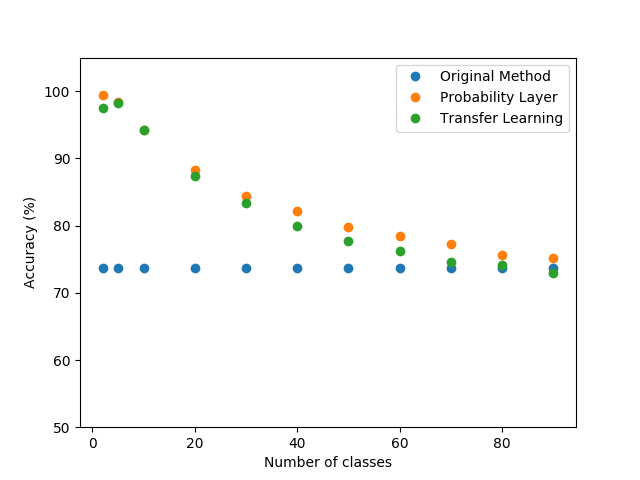
\includegraphics[width=\textwidth]{PLvsRetrain.png}
        \caption{Various number of classes}
        \label{fig:complexNumber}
    \end{subfigure}
    ~ %add desired spacing between images, e. g. ~, \quad, \qquad, \hfill etc. 
      %(or a blank line to force the subfigure onto a new line)
    \begin{subfigure}[b]{0.49\textwidth}
        \centering
        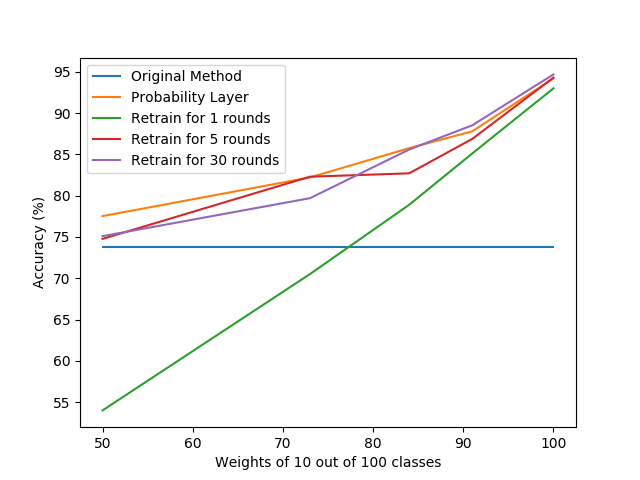
\includegraphics[width=\textwidth]{VaryingDistribution.png}
        \caption{Ten classes occupying various percentage}
        \label{fig:complexDistribution}
    \end{subfigure}
    \caption{Probability layer on denseNet}\label{fig:complex}
\end{figure}

% Third paragraph: Experiment setting
We evaluate probability layer's ability in making use of environment on number of classes as well as in-class distribution when number of classes is fixed. The dataset is a subset of CIFAR100 \cite{krizhevsky2009learning}. CIFAR100 \cite{krizhevsky2009learning} is a dataset with 100 classes and each class has 500 training images and 100 testing images. We trained denseNet \cite{huang2017densely} on original CIFAR100 training datasets. For testing part, to evaluate the performance of probability layer under various conditions, we choose a subset of testing images as the new testing dataset. For various number of classes, we select a subset of classes and each class has equal number of images. For testing the ability to adapt to a dataset with a few major classes and many minor classes, we choose $10$ classes as the major class, select all $100$ testing images for each class, and randomly choose a fixed number of testing images in other $90$ classes, according to the desired percentage that $10$ major classes occupy. For implementing probability layer, we calculate the percentage of every class in the generated testing dataset and set up the parameters in probability layer correspondingly. When implementing transfer learning, we use the same model trained on CIFAR100 and retrain on the same generated training dataset. For the retraining process, we retrain all fully-connected layers after convolutional layers, since this is the method reported to have best accuracy gain (CITATIONS). In the retraining process, various epoches were used, i.e. $1$, $5$, $30$. The maximum epoch tried is $30$ because we consider both latency and energy which could be used in normal operation instead of retraining. For example, if the generated training dataset has 10 classes and 500 images in each class, retraining for $30$ epochs means that $150,000$ images will be processed by the models. Since generally the image will be processed every one second, the machine can proceed around $41$ more hours without so many retraining.

% Forth paragraph: Show probability layer works on complex models
Fig. \ref{fig:complexNumber} shows the comparison between probability layer and transfer learning on various number of classes. Original model represents the model with neither probability layer nor transfer learning, i.e. without adaption to the new dataset. We can find that the model with probability layer performs consistently better than the model without probability layer. When number of classes is less than $10$, probability layer can boost the top-1 accuracy to be more than 95\%, which is better than the human's ability in recognition, reported to be a top-5 error of 5.1\% \cite{russakovsky2015imagenet}. When number of classes is less than 10, probability layer's performance is at most 2\% lower than retraining for $5$ rounds. As number of classes becomes larger than $10$, probability layer would always perform better than retraining for $5$ rounds. The advantage of probability layer over retraining increases as number of classes increases. One point worth noting is that when the number of classes increases over $90$, retraining would bring worse accuracy than original model without retraining. In contrast, the probability layer can still bring 2\% advantage over original model. All these observations indicate that probability layer has better ability in using various environment, especially when the number of classes gets larger.

Fig. \ref{fig:complexNumber} shows the accuracy on testing data when there are $10$ major classes occupying various weights among $100$ classes. The other $90$ classes are minor classes with same weights. While the weights increase from $50$\% to $100$\%, probability layer performs consistently better than the retraining for $5$ or $1$ rounds. Even if we retrain the model for $30$ rounds, probability layer still performs better when weights of $10$ major classes is less than $85$\%. When the weights increase over $85$\%, the advantage of retraining for $30$ rounds over probability layer is at most $0.5$\%. Retraining for $30$ rounds takes $60$ seconds and xxx GFLOPS. Considering the intensive energy-consumption and time latency of retraining for $30$ rounds, this benefit of $0.5$\% advantage is not so significant. We should also note that retraining for $30$ rounds would make the accuracy to be much lower than original model when weights of major classes is less than 75\%. Since we need to choose a method before we start in automatically using environment information, we can conclude that probability layer is the most suitable method.

% Fifth paragraph: show probability layer not work on simple model
Although probability layer boost the top-1 accuracy of complex model a lot, shallow models cannot get the same benefits. We train a shallow model with $4$ convolutional layers and $3$ fully connected layers on CIFAR100 and test the model with probability layer on a generated dataset with $10$ classes and each class has $500$ images. Without probability layer, the accuracy is 30\%. The accuracy will only increase 2\% when adding probability layer. IN contrast, if we both train and test on the generated dataset, the accuracy is 55\%. From these results, we can find that implementing rescaling does not guarantee a same performance with transfer learning. We will give a detailed analysis on the intuition behind the probability layer and provide a guidance on which model probability layer can bring benefit.



}




\section{Analysis on Logits}
% First paragraph: Discuss the intuition behind the probability layer and why it sometimes works and sometimes not. Introduce the importance of logits and give a summary



% Second paragraph: Present the logits of simple models



% Third paragraph: Present the logits of complex models


% Forth paragraph: Introduce the metric for whether model is confident about its prediction



% Fifth paragraph: Introduce the metric for whether a model can benefit from probability layer.


\section{Experiments}
\textit{Probability layer} is an extra layer after the softmax layer in the CNN models. With \textit{probability layer}, we can use runtime class distribution without retraining. As we have discussed previously, there are gains in both reducing energy consumption and time latency. Existing methods, i.e. retraining last few layers, requires thousands of images to go through the network for tens of rounds, which waste lots of energy. The retraining also takes time and introduce several seconds latency during which new images cannot be processed. With \textit{probability layer}, all of these inconvenience will be avoided and better performance will be gained. Thus \textit{probability layer} is a brilliant supplement or even replacement of retraining last few layers.

To implement probability layer, the only thing we need to do is to add an extra layer after the softmax layer. Originally, the last layer of CNN model is softmax layer. The output of softmax layer is a vector $(p_1, p_2, ..., p_n)$, where $n$ is the number of nodes in the softmax layer, i.e. the number of classes that the CNN model wants to predict from. Also, $p_1$, ..., $p_n$ is a series of numbers between $0$nd $1$. Thus we would treat $p_i$ as the probability that indicates how likely an image may belong to a specific class $i$. The main idea of probability layer is to add a constant to classes that is more likely to be the true label according to the runtime distribution. For example, if the runtime distribution shows that only the first 10 out of 100 classes could appear in a context, the probability layer will add a constant to $p_1$, ..., $p_{10}$, the predicted probability of these 10 classes. In other word, in this case, the probability layer is $ c_1, c_2, c_3, c_4, c_5, c_6, c_7, c_8, c_9, c_{10}, 0, ...,0 )$, where $c_i$ is a constant between $0$ and $1$ and the output of the probability layer is $(p_1 + c_1, p_2 + c_2, ..., p_{10}+c_{10}, p_{11}, ..., p_{100})$. Here we treat $c_i$ as hyper-parameters. The larger the $c_i$ is, the stronger confidence we have in runtime distribution.

The success of probability layer depends on the accuracy of original model. Intuitively, adding a constant to a set of domain classes according to the run-time distribution would encourage the model to select among these domain classes. If the original model is precise, i.e. have high top-5 accuracy, this constrain could rule out some classes and help the model to get a correct result. For example, if the output of softmax layer is $(0.3, 0, ..., 0, 0.7)$ and the probability layer according to runtime distribution is $(0.5, 0.5, 0.5, 0.5, 0.5, 0, ..., 0)$, the output of probability layer would be $(0.8, 0.5, 0.5, 0.5, 0.5, 0, ..., 0.7)$. Assume the correct label is $0$,  the prediction without probability layer is $99$, which is wrong, and the prediction with probability layer is $0$, which is correct. In this case, probability layer helps us to rule out the unlikely class $99$.

A possible case is that the probability corresponding to the true label are not highest even in domain classes. In this case, the probability will not be helpful. We found that top-5 accuracy is a good meric to measure how well the probability layer could help the original model. In other word, the benefit of probability layer is to improve the top-1 accuracy to be as large as the top-5 accuracy. If the top-5 accuracy is very high, the true label would have the top-5 high probability. The probability layer will constrain the predicted label to be the intersection between these top-5 labels and the domain labels according to runtime distribution. Thus we can increase top-1 accuracy toward top-5 accuracy. 

However, if the number of domain classes are 5 and the top-5 accuracy of the model is low, it is possible that the probability of true label is not the highest among the 5 domain classes. In this case, the benefit of probability layer would be slight. Thus, the higher top-5 accuracy the original model have, the better effect the probability layer would bring. In other word, if we use probability layer on a model with low top-5 accuracy, the benefit would be small. 

A series of experiments on various kind of specialized datasets have shown the effectiveness of probability layer. CIFAR100 is a prevalent benchmark for various kind of CNN models, which has 100 classes, a training dataset with 500 images per class, and a testing dataset with 100 images per class. To mimic the runtime distribution, we generate a specialized dataset manually. For example, in generation of a specialized dataset with 80\% data skew and 10 domain classes, we would use 1000 images from the testing dataset according to these 10 domain classes, and randomly select 250 images from other classes. We trained the model on original CIFAR100 training dataset and test the model on various kind of specialized datasets with different number of domain classes and selection of domain classes. We also take into account that the selection of domain classes because the choice of labels have strong effect on the test accuracy, even if we keep the number of domain classes unchanged. Actually some classes are easier to classify than others. To eliminate this random effect, we will choose different groups of labels for each number of domain classes.

Figure \ref{fig:ProbabilityLayer} summarizes the results. As a benchmark, the test accuracy on the CIFAR100 testing dataset without probability layer is 73.74\%. If the number of domain classes is 2 and we choose the label 0 and 1, the accuracy without probability layer is 88.12\%. The difference between specialized testing accuracy 88.12\% and the overall accuracy 73.74\% is due to selection of classes. If we change the label pair from (0,1) to (3,5), the accuracy would also change from 88.12\% to 61.39\%. However, in both case, the accuracy with probability layer are 98.51\% and 99.01\%, which performs very well consistently. 

Then we increase the number of domain classes from 2 to 5 and choose domain classes as 0 to 4 and 5 to 9 respectively. This time, the effectiveness of selection of domain classes appears again. If we set domain classes as 0 to 4, the accuracy without probability layer would be 66.33\%. If we set domain classes as 5 to 9, the accuracy would be 81.06\%. The accuracy with probability layer in these two cases would be 93.03\% and 97.01\% respectively. The benefit of probability layer are 26.70\% and 15.95\% respectively.

When we increase the number of domain classes further to 10, the effectiveness of probability layer would still be dramatic. We choose 0 to 9, 10 to 19, 20 to 29 as domain classes. The accuracy without probability layer would be 75.35\%, 67.16\%, and 75.84\%. The accuracy with probability layer would be 94.21\%, 91.41\%, and 92.22\%. The benefits are 18.86\%, 24.26\%, and 16.38\%.

To explore the interaction between probability layer and number of domain classes, we increase the number of domain classes gradually from 2 to 100. The benefit disappears gracefully. When number of domain classes is less than 20, the benefit are above 18\%. Even if we have 40 domain classes, the benefit is still around 10\%. When there are 60 classes, there are 5\% benefit. Since we do not need retrain, these benefit are almost free. We do not need extra memory or energy and we have not introduced any extra latency. The only thing that we need is the run time distribution, which could be collected easily through an in-memory record.


\begin{figure}
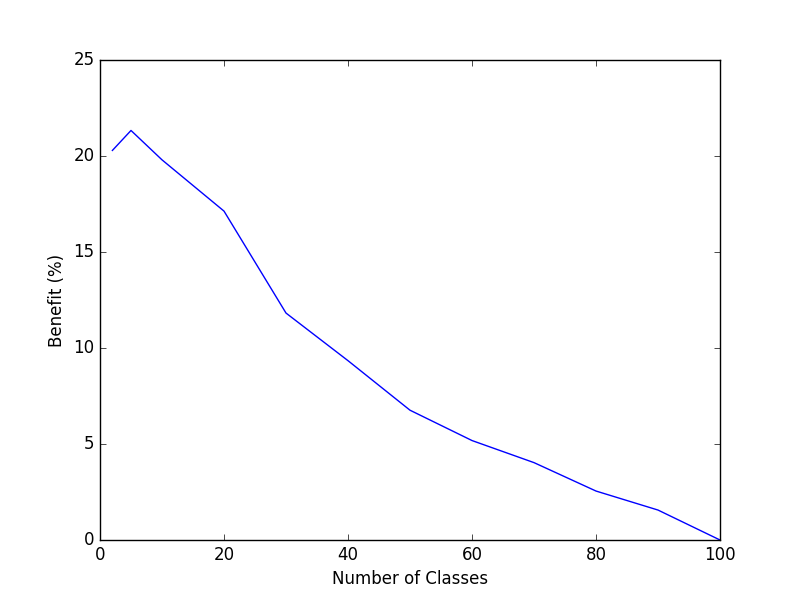
\includegraphics[scale=0.43]{figure_1.png}
\caption{Probability Layer Result}
\label{fig:ProbabilityLayer}
\end{figure}


\begin{table*}[!th]
    \centering
    \begin{tabular}{l|c|c|c}
        \hline
        \multicolumn{1}{c|}{Test Data} & Parameter  & Accuracy & Benefit \\
        Original CIFAR100 & 0 & 73.74\% &  \\
        \hline
        2 classes (0, 1) & 0 & 88.12\% &  \\
        2 classes (0, 1) & 1.0 & 98.51\% & +10.39\% \\
        \hline
        2 classes (3, 5) & 0 & 61.39\% &  \\
        2 classes (3, 5) & 1.0 & 99.01\% & +37.62\% \\
        \hline
        2 classes (0, 99) & 0 & 84.65\% & \\
        2 classes (0, 99) & 1.0 & 97.52\% & +12.87\% \\
        \hline
        5 classes $(0, ..., 4)$ & 0 & 66.33\% &  \\
        5 classes $(0, ..., 4)$ & 1.0 & 93.03\% & +26.70\% \\
        \hline
        5 classes $(5, ..., 9)$ & 0 & 81.06\% &  \\
        5 classes $(5, ..., 9)$ & 1.0 & 97.01\% & +15.95\% \\
        \hline
        10 classes $(0, ..., 9)$ & 0 & 75.35\% &  \\
        10 classes $(0, ..., 0)$ & 1.0 & 94.21\% & +18.86\% \\
        \hline
        10 classes $(10, ..., 19)$ & 0 & 67.16\% &  \\
        10 classes $(10, ..., 19)$ & 1.0 & 91.42\% & +24.26\% \\
        \hline
        10 classes $(20, ..., 29)$ & 0 & 75.84\% &  \\
        10 classes $(20, ..., 29)$ & 1.0 & 92.22\% & +16.38\% \\
        \hline
        
        
    \end{tabular}
    \vspace{1em}
    \caption{Test Probability Layer on Different Locality}
    \label{tab:ProbabilityLayer1}
\end{table*}




\subsection{Comparison with naive mask}
A naive replacement of \textit{probability layer} is to mask all non-domain classes, called \textit{naive mask}. Probability layer is a generalization of naive mask. In fact, naive mask is equivalent to set the parameter $c$ in probability layer to be $1.0$. The intuitive explanation of naive mask is to only have nodes according to the main classes since the predicted label could only be one of these domain classes. If we use naive mask, all the prediction of images with classes besides the main classes would be wrong. This would limit the usage of naive mask dramatically. For example, if the domain classes occupy 70\% in the runtime distribution, the accuracy with naive mask would be less than 70\%, which is smaller than the accuracy without naive mask and makes naive mask useless, even if 70\% skew is not a low skew in daily life. 

Probability layer can avoid this problem if we set the parameter c to be strictly less than 1.0. This benefit depends on high accuracy of original model again. Generally, in denseNet, if an image could be classified correctly, the probability corresponding to the correct label after softmax layer is 1, and the probability corresponding to other labels are almost 0. For example, if the true label of an image is $11$, the output of softmax would generally be $(0, 0, 0, 0, 0, 0, 0, 0, 0, 0, 1, 0, 0, 0, 0, ... 0)$. Even if we add a probability layer to first 10 classes and use the parameter as 0.9, the output would be $(0.9, 0.9, 0.9, 0.9, 0.9, 0.9, 0.9, 0.9, 0.9, 0.9, 1, 0, 0, 0, 0, ... 0)$. In this case, the model would still mark $11$ as the correct label and the probability layer has no bad effect. However, if we use naive mask to rule out all classes other than first ten classes, the prediction would be constrained in the first ten classes and will be wrong. 

In other words, the probability layer only has bad effect when the original model is not quite sure about how to classify an image. For example, if the true label of an image is 11, the output might be $(0.3, 0, 0, 0, 0, 0, 0, 0, 0, 0, 0.7, 0, 0, 0, 0, ... 0)$. After we add the probability layer to first 10 classes and use the parameter as 0.9, the output would be $(1.2, 0.9, 0.9, 0.9, 0.9, 0.9, 0.9, 0.9, 0.9, 0.9, 0.7, 0, 0, 0, 0, ... 0)$. In this case, the model would mark 1 as the correct label and the probability layer have a bad effect. However, the happen of this bad effect needs two conditions. First, the labels with predicted probability 0.3 and 0.7 also appear in the first ten classes. Second, the predicted probability of true label is lower than the other one. Actually this is a rare case.

We have also done some experiments to support our result. Figure \ref{fig:NaiveMask} shows the comparison between probability layer and naive mask under different configurations. The red dash line represents the original accuracy without probability layer and naive mask, which is 74.57\%. When the number of domain classes is 10 and the distribution skew is 50\%, the accuracy with probability layer is 75.28\%, while the accuracy with naive mask is only 47.49\%. Thus probability layer has a positive effect even if the distribution skew is only 50\%, while the naive mask has a strong negative effect in this context. As we increase distribution skew gradually, the accuracy with probability layer and naive mask keeps increasing. Only after the distribution skew becomes larger than 77.67\%, naive mask starts to show positive effect on accuracy while probability layer keeps showing positive effect in all settings. As distribution skew approaches 100\%, the effect of naive mask catches probability layer up, since the true labels start to only exist in domain classes. In short, probability layer is a generalization of naive mask and shows benefit over original model and naive mask consistently.

\begin{figure}
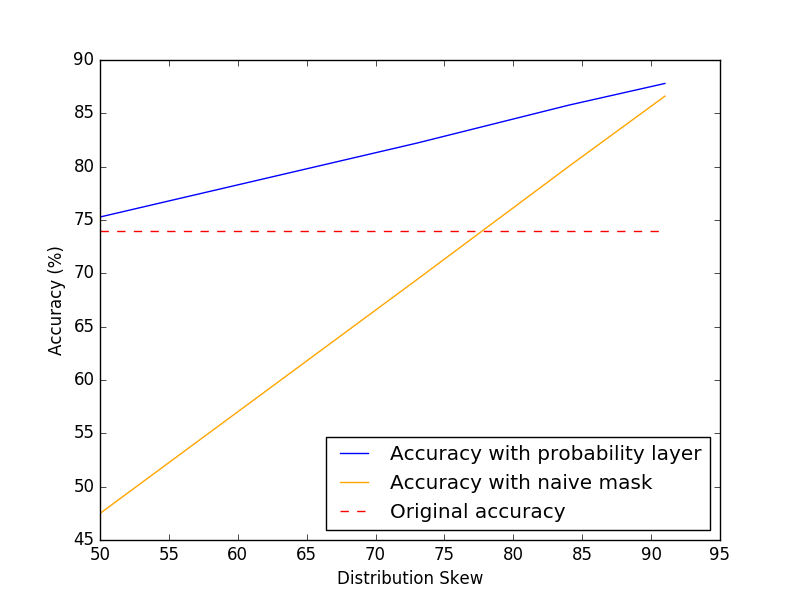
\includegraphics[scale=0.43]{figure_1-1.png}
\caption{Comparison Between Probability Layer and Naive Mask}
\label{fig:NaiveMask}
\end{figure}



\bibliography{nips_2018}
\bibliographystyle{plain}


\end{document}
